
% Default to the notebook output style

    


% Inherit from the specified cell style.




    
\documentclass{article}

    
    
    \usepackage{graphicx} % Used to insert images
    \usepackage{adjustbox} % Used to constrain images to a maximum size 
    \usepackage{color} % Allow colors to be defined
    \usepackage{enumerate} % Needed for markdown enumerations to work
    \usepackage{geometry} % Used to adjust the document margins
    \usepackage{amsmath} % Equations
    \usepackage{amssymb} % Equations
    \usepackage{eurosym} % defines \euro
    \usepackage[mathletters]{ucs} % Extended unicode (utf-8) support
    \usepackage[utf8x]{inputenc} % Allow utf-8 characters in the tex document
    \usepackage{fancyvrb} % verbatim replacement that allows latex
    \usepackage{grffile} % extends the file name processing of package graphics 
                         % to support a larger range 
    % The hyperref package gives us a pdf with properly built
    % internal navigation ('pdf bookmarks' for the table of contents,
    % internal cross-reference links, web links for URLs, etc.)
    \usepackage{hyperref}
    \usepackage{longtable} % longtable support required by pandoc >1.10
    \usepackage{booktabs}  % table support for pandoc > 1.12.2
    \usepackage{indentfirst}
    \usepackage{floatrow}
    
    
    \definecolor{orange}{cmyk}{0,0.4,0.8,0.2}
    \definecolor{darkorange}{rgb}{.71,0.21,0.01}
    \definecolor{darkgreen}{rgb}{.12,.54,.11}
    \definecolor{myteal}{rgb}{.26, .44, .56}
    \definecolor{gray}{gray}{0.45}
    \definecolor{lightgray}{gray}{.95}
    \definecolor{mediumgray}{gray}{.8}
    \definecolor{inputbackground}{rgb}{.95, .95, .85}
    \definecolor{outputbackground}{rgb}{.95, .95, .95}
    \definecolor{traceback}{rgb}{1, .95, .95}
    % ansi colors
    \definecolor{red}{rgb}{.6,0,0}
    \definecolor{green}{rgb}{0,.65,0}
    \definecolor{brown}{rgb}{0.6,0.6,0}
    \definecolor{blue}{rgb}{0,.145,.698}
    \definecolor{purple}{rgb}{.698,.145,.698}
    \definecolor{cyan}{rgb}{0,.698,.698}
    \definecolor{lightgray}{gray}{0.5}
    
    % bright ansi colors
    \definecolor{darkgray}{gray}{0.25}
    \definecolor{lightred}{rgb}{1.0,0.39,0.28}
    \definecolor{lightgreen}{rgb}{0.48,0.99,0.0}
    \definecolor{lightblue}{rgb}{0.53,0.81,0.92}
    \definecolor{lightpurple}{rgb}{0.87,0.63,0.87}
    \definecolor{lightcyan}{rgb}{0.5,1.0,0.83}
    
    % commands and environments needed by pandoc snippets
    % extracted from the output of `pandoc -s`
    \providecommand{\tightlist}{%
      \setlength{\itemsep}{0pt}\setlength{\parskip}{0pt}}
    \DefineVerbatimEnvironment{Highlighting}{Verbatim}{commandchars=\\\{\}}
    % Add ',fontsize=\small' for more characters per line
    \newenvironment{Shaded}{}{}
    \newcommand{\KeywordTok}[1]{\textcolor[rgb]{0.00,0.44,0.13}{\textbf{{#1}}}}
    \newcommand{\DataTypeTok}[1]{\textcolor[rgb]{0.56,0.13,0.00}{{#1}}}
    \newcommand{\DecValTok}[1]{\textcolor[rgb]{0.25,0.63,0.44}{{#1}}}
    \newcommand{\BaseNTok}[1]{\textcolor[rgb]{0.25,0.63,0.44}{{#1}}}
    \newcommand{\FloatTok}[1]{\textcolor[rgb]{0.25,0.63,0.44}{{#1}}}
    \newcommand{\CharTok}[1]{\textcolor[rgb]{0.25,0.44,0.63}{{#1}}}
    \newcommand{\StringTok}[1]{\textcolor[rgb]{0.25,0.44,0.63}{{#1}}}
    \newcommand{\CommentTok}[1]{\textcolor[rgb]{0.38,0.63,0.69}{\textit{{#1}}}}
    \newcommand{\OtherTok}[1]{\textcolor[rgb]{0.00,0.44,0.13}{{#1}}}
    \newcommand{\AlertTok}[1]{\textcolor[rgb]{1.00,0.00,0.00}{\textbf{{#1}}}}
    \newcommand{\FunctionTok}[1]{\textcolor[rgb]{0.02,0.16,0.49}{{#1}}}
    \newcommand{\RegionMarkerTok}[1]{{#1}}
    \newcommand{\ErrorTok}[1]{\textcolor[rgb]{1.00,0.00,0.00}{\textbf{{#1}}}}
    \newcommand{\NormalTok}[1]{{#1}}
    
    % Define a nice break command that doesn't care if a line doesn't already
    % exist.
    \def\br{\hspace*{\fill} \\* }
    % Math Jax compatability definitions
    \def\gt{>}
    \def\lt{<}
    % Document parameters
    \title{Homework 5}
    \author{Roly Vicar\'ia \\ STAT501 Fall 2015}   
    

    % Pygments definitions
    
\makeatletter
\def\PY@reset{\let\PY@it=\relax \let\PY@bf=\relax%
    \let\PY@ul=\relax \let\PY@tc=\relax%
    \let\PY@bc=\relax \let\PY@ff=\relax}
\def\PY@tok#1{\csname PY@tok@#1\endcsname}
\def\PY@toks#1+{\ifx\relax#1\empty\else%
    \PY@tok{#1}\expandafter\PY@toks\fi}
\def\PY@do#1{\PY@bc{\PY@tc{\PY@ul{%
    \PY@it{\PY@bf{\PY@ff{#1}}}}}}}
\def\PY#1#2{\PY@reset\PY@toks#1+\relax+\PY@do{#2}}

\expandafter\def\csname PY@tok@gd\endcsname{\def\PY@tc##1{\textcolor[rgb]{0.63,0.00,0.00}{##1}}}
\expandafter\def\csname PY@tok@gu\endcsname{\let\PY@bf=\textbf\def\PY@tc##1{\textcolor[rgb]{0.50,0.00,0.50}{##1}}}
\expandafter\def\csname PY@tok@gt\endcsname{\def\PY@tc##1{\textcolor[rgb]{0.00,0.27,0.87}{##1}}}
\expandafter\def\csname PY@tok@gs\endcsname{\let\PY@bf=\textbf}
\expandafter\def\csname PY@tok@gr\endcsname{\def\PY@tc##1{\textcolor[rgb]{1.00,0.00,0.00}{##1}}}
\expandafter\def\csname PY@tok@cm\endcsname{\let\PY@it=\textit\def\PY@tc##1{\textcolor[rgb]{0.25,0.50,0.50}{##1}}}
\expandafter\def\csname PY@tok@vg\endcsname{\def\PY@tc##1{\textcolor[rgb]{0.10,0.09,0.49}{##1}}}
\expandafter\def\csname PY@tok@m\endcsname{\def\PY@tc##1{\textcolor[rgb]{0.40,0.40,0.40}{##1}}}
\expandafter\def\csname PY@tok@mh\endcsname{\def\PY@tc##1{\textcolor[rgb]{0.40,0.40,0.40}{##1}}}
\expandafter\def\csname PY@tok@go\endcsname{\def\PY@tc##1{\textcolor[rgb]{0.53,0.53,0.53}{##1}}}
\expandafter\def\csname PY@tok@ge\endcsname{\let\PY@it=\textit}
\expandafter\def\csname PY@tok@vc\endcsname{\def\PY@tc##1{\textcolor[rgb]{0.10,0.09,0.49}{##1}}}
\expandafter\def\csname PY@tok@il\endcsname{\def\PY@tc##1{\textcolor[rgb]{0.40,0.40,0.40}{##1}}}
\expandafter\def\csname PY@tok@cs\endcsname{\let\PY@it=\textit\def\PY@tc##1{\textcolor[rgb]{0.25,0.50,0.50}{##1}}}
\expandafter\def\csname PY@tok@cp\endcsname{\def\PY@tc##1{\textcolor[rgb]{0.74,0.48,0.00}{##1}}}
\expandafter\def\csname PY@tok@gi\endcsname{\def\PY@tc##1{\textcolor[rgb]{0.00,0.63,0.00}{##1}}}
\expandafter\def\csname PY@tok@gh\endcsname{\let\PY@bf=\textbf\def\PY@tc##1{\textcolor[rgb]{0.00,0.00,0.50}{##1}}}
\expandafter\def\csname PY@tok@ni\endcsname{\let\PY@bf=\textbf\def\PY@tc##1{\textcolor[rgb]{0.60,0.60,0.60}{##1}}}
\expandafter\def\csname PY@tok@nl\endcsname{\def\PY@tc##1{\textcolor[rgb]{0.63,0.63,0.00}{##1}}}
\expandafter\def\csname PY@tok@nn\endcsname{\let\PY@bf=\textbf\def\PY@tc##1{\textcolor[rgb]{0.00,0.00,1.00}{##1}}}
\expandafter\def\csname PY@tok@no\endcsname{\def\PY@tc##1{\textcolor[rgb]{0.53,0.00,0.00}{##1}}}
\expandafter\def\csname PY@tok@na\endcsname{\def\PY@tc##1{\textcolor[rgb]{0.49,0.56,0.16}{##1}}}
\expandafter\def\csname PY@tok@nb\endcsname{\def\PY@tc##1{\textcolor[rgb]{0.00,0.50,0.00}{##1}}}
\expandafter\def\csname PY@tok@nc\endcsname{\let\PY@bf=\textbf\def\PY@tc##1{\textcolor[rgb]{0.00,0.00,1.00}{##1}}}
\expandafter\def\csname PY@tok@nd\endcsname{\def\PY@tc##1{\textcolor[rgb]{0.67,0.13,1.00}{##1}}}
\expandafter\def\csname PY@tok@ne\endcsname{\let\PY@bf=\textbf\def\PY@tc##1{\textcolor[rgb]{0.82,0.25,0.23}{##1}}}
\expandafter\def\csname PY@tok@nf\endcsname{\def\PY@tc##1{\textcolor[rgb]{0.00,0.00,1.00}{##1}}}
\expandafter\def\csname PY@tok@si\endcsname{\let\PY@bf=\textbf\def\PY@tc##1{\textcolor[rgb]{0.73,0.40,0.53}{##1}}}
\expandafter\def\csname PY@tok@s2\endcsname{\def\PY@tc##1{\textcolor[rgb]{0.73,0.13,0.13}{##1}}}
\expandafter\def\csname PY@tok@vi\endcsname{\def\PY@tc##1{\textcolor[rgb]{0.10,0.09,0.49}{##1}}}
\expandafter\def\csname PY@tok@nt\endcsname{\let\PY@bf=\textbf\def\PY@tc##1{\textcolor[rgb]{0.00,0.50,0.00}{##1}}}
\expandafter\def\csname PY@tok@nv\endcsname{\def\PY@tc##1{\textcolor[rgb]{0.10,0.09,0.49}{##1}}}
\expandafter\def\csname PY@tok@s1\endcsname{\def\PY@tc##1{\textcolor[rgb]{0.73,0.13,0.13}{##1}}}
\expandafter\def\csname PY@tok@kd\endcsname{\let\PY@bf=\textbf\def\PY@tc##1{\textcolor[rgb]{0.00,0.50,0.00}{##1}}}
\expandafter\def\csname PY@tok@sh\endcsname{\def\PY@tc##1{\textcolor[rgb]{0.73,0.13,0.13}{##1}}}
\expandafter\def\csname PY@tok@sc\endcsname{\def\PY@tc##1{\textcolor[rgb]{0.73,0.13,0.13}{##1}}}
\expandafter\def\csname PY@tok@sx\endcsname{\def\PY@tc##1{\textcolor[rgb]{0.00,0.50,0.00}{##1}}}
\expandafter\def\csname PY@tok@bp\endcsname{\def\PY@tc##1{\textcolor[rgb]{0.00,0.50,0.00}{##1}}}
\expandafter\def\csname PY@tok@c1\endcsname{\let\PY@it=\textit\def\PY@tc##1{\textcolor[rgb]{0.25,0.50,0.50}{##1}}}
\expandafter\def\csname PY@tok@kc\endcsname{\let\PY@bf=\textbf\def\PY@tc##1{\textcolor[rgb]{0.00,0.50,0.00}{##1}}}
\expandafter\def\csname PY@tok@c\endcsname{\let\PY@it=\textit\def\PY@tc##1{\textcolor[rgb]{0.25,0.50,0.50}{##1}}}
\expandafter\def\csname PY@tok@mf\endcsname{\def\PY@tc##1{\textcolor[rgb]{0.40,0.40,0.40}{##1}}}
\expandafter\def\csname PY@tok@err\endcsname{\def\PY@bc##1{\setlength{\fboxsep}{0pt}\fcolorbox[rgb]{1.00,0.00,0.00}{1,1,1}{\strut ##1}}}
\expandafter\def\csname PY@tok@mb\endcsname{\def\PY@tc##1{\textcolor[rgb]{0.40,0.40,0.40}{##1}}}
\expandafter\def\csname PY@tok@ss\endcsname{\def\PY@tc##1{\textcolor[rgb]{0.10,0.09,0.49}{##1}}}
\expandafter\def\csname PY@tok@sr\endcsname{\def\PY@tc##1{\textcolor[rgb]{0.73,0.40,0.53}{##1}}}
\expandafter\def\csname PY@tok@mo\endcsname{\def\PY@tc##1{\textcolor[rgb]{0.40,0.40,0.40}{##1}}}
\expandafter\def\csname PY@tok@kn\endcsname{\let\PY@bf=\textbf\def\PY@tc##1{\textcolor[rgb]{0.00,0.50,0.00}{##1}}}
\expandafter\def\csname PY@tok@mi\endcsname{\def\PY@tc##1{\textcolor[rgb]{0.40,0.40,0.40}{##1}}}
\expandafter\def\csname PY@tok@gp\endcsname{\let\PY@bf=\textbf\def\PY@tc##1{\textcolor[rgb]{0.00,0.00,0.50}{##1}}}
\expandafter\def\csname PY@tok@o\endcsname{\def\PY@tc##1{\textcolor[rgb]{0.40,0.40,0.40}{##1}}}
\expandafter\def\csname PY@tok@kr\endcsname{\let\PY@bf=\textbf\def\PY@tc##1{\textcolor[rgb]{0.00,0.50,0.00}{##1}}}
\expandafter\def\csname PY@tok@s\endcsname{\def\PY@tc##1{\textcolor[rgb]{0.73,0.13,0.13}{##1}}}
\expandafter\def\csname PY@tok@kp\endcsname{\def\PY@tc##1{\textcolor[rgb]{0.00,0.50,0.00}{##1}}}
\expandafter\def\csname PY@tok@w\endcsname{\def\PY@tc##1{\textcolor[rgb]{0.73,0.73,0.73}{##1}}}
\expandafter\def\csname PY@tok@kt\endcsname{\def\PY@tc##1{\textcolor[rgb]{0.69,0.00,0.25}{##1}}}
\expandafter\def\csname PY@tok@ow\endcsname{\let\PY@bf=\textbf\def\PY@tc##1{\textcolor[rgb]{0.67,0.13,1.00}{##1}}}
\expandafter\def\csname PY@tok@sb\endcsname{\def\PY@tc##1{\textcolor[rgb]{0.73,0.13,0.13}{##1}}}
\expandafter\def\csname PY@tok@k\endcsname{\let\PY@bf=\textbf\def\PY@tc##1{\textcolor[rgb]{0.00,0.50,0.00}{##1}}}
\expandafter\def\csname PY@tok@se\endcsname{\let\PY@bf=\textbf\def\PY@tc##1{\textcolor[rgb]{0.73,0.40,0.13}{##1}}}
\expandafter\def\csname PY@tok@sd\endcsname{\let\PY@it=\textit\def\PY@tc##1{\textcolor[rgb]{0.73,0.13,0.13}{##1}}}

\def\PYZbs{\char`\\}
\def\PYZus{\char`\_}
\def\PYZob{\char`\{}
\def\PYZcb{\char`\}}
\def\PYZca{\char`\^}
\def\PYZam{\char`\&}
\def\PYZlt{\char`\<}
\def\PYZgt{\char`\>}
\def\PYZsh{\char`\#}
\def\PYZpc{\char`\%}
\def\PYZdl{\char`\$}
\def\PYZhy{\char`\-}
\def\PYZsq{\char`\'}
\def\PYZdq{\char`\"}
\def\PYZti{\char`\~}
% for compatibility with earlier versions
\def\PYZat{@}
\def\PYZlb{[}
\def\PYZrb{]}
\makeatother


    % Exact colors from NB
    \definecolor{incolor}{rgb}{0.0, 0.0, 0.5}
    \definecolor{outcolor}{rgb}{0.545, 0.0, 0.0}



    
    % Prevent overflowing lines due to hard-to-break entities
    \sloppy 
    % Setup hyperref package
    \hypersetup{
      breaklinks=true,  % so long urls are correctly broken across lines
      colorlinks=true,
      urlcolor=blue,
      linkcolor=darkorange,
      citecolor=darkgreen,
      }
    % Slightly bigger margins than the latex defaults
    
    \geometry{verbose,tmargin=1in,bmargin=1in,lmargin=1in,rmargin=1in}
    
    

    \begin{document}
    
    
    \maketitle
    
    

    
    \subsubsection{Question 1}\label{question-1}

\begin{enumerate}
\def\labelenumi{\alph{enumi})}
\item
  Based on the plot, I would say that there is no correlation between
  ingredA and ingredB. You can see the fixed points corresponding to all
  the possible combinations of ingredA (1, 2, 3) and ingredB (1, 2, 3,
  4). 
  
  \begin{figure}[h!]
 \centering
 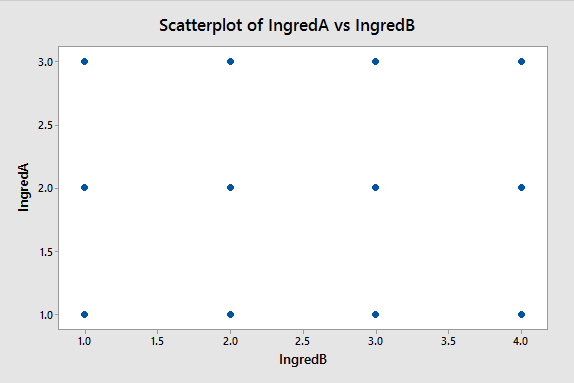
\includegraphics[scale=.5]{./images/scatterplot_ingredA-vs-ingredB.png}
 % scatterplot_ingredA-vs-ingredB.png: 574x383 pixel, 96dpi, 15.19x10.13 cm, bb=0 0 430 287
\end{figure}

\item
  The plot of ingredA vs Yield shows a slight indication of a positive
  linear relationship. It's not a strong one because the Yield has a lot
  of variability for each level of ingredA. The plot of ingredB vs Yield
  appears to have a stronger positive correlation. It looks to me that
  ingredB is a stronger predictor. 
  
  \begin{figure}[!h]
   \begin{floatrow}
    \ffigbox{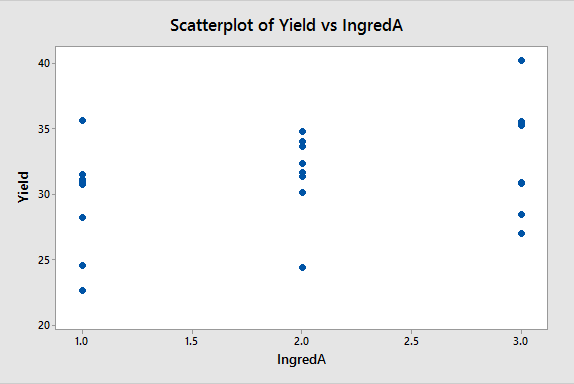
\includegraphics[scale=0.5]{./images/scatterplot_ingredA-vs-Yield.png}}{}
   \ffigbox{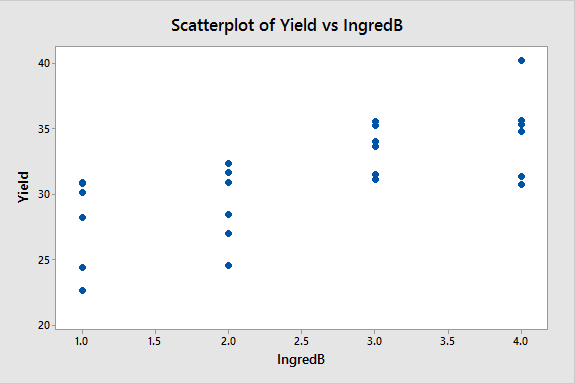
\includegraphics[scale=0.5]{./images/scatterplot_ingredB-vs-Yield.png}}{}
  \end{floatrow}

  \end{figure}

  \newpage
\item
  \(Yield = 27.75 + 1.763 IngredA\)

  \begin{enumerate}
  \def\labelenumii{\roman{enumii})}
  \tightlist
  \item
    The slope is 1.763. This can be interpreted as saying that
    increasing ingredA by 1 unit would increase yield by about 1.763
    units.
  \item
    The \(R^2\) value is 13.05\%
  \item
    The \(p\)-value of the regression is .083 which indicates that it
    may not be statistically significant.
  \end{enumerate}
\item
  \(Yield = 25.07 + 2.482 IngredB\)

  \begin{enumerate}
  \def\labelenumii{\roman{enumii})}
  \tightlist
  \item
    The slope is 2.482. This can be interpreted as saying that
    increasing ingredB by 1 unit would increase yield by about 2.482
    units.
  \item
    The \(R^2\) value is 48.50\%
  \item
    The \(p\)-value of the regression is is 0.000 which indicates it is
    statistically significant.
  \end{enumerate}
\item
  \(Yield = 21.54 + 1.763 IngredA + 2.482 IngredB\)

  \begin{enumerate}
  \def\labelenumii{\roman{enumii})}
  \tightlist
  \item
    The values of the coefficients are 1.763 and 2.482. This occurs
    because ingredA and ingredB are not correlated.
  \item
    The \(R^2\) value is 61.55\%. This is indeed equal to the sum of
    13.05\% and 48.5\%. This occurs for the same reason as part (i),
    namely that the two predictor variables are not correlated.
  \item
    In the multiple regression, ingredA has a \(p\)-value of .014, which
    is statistically significant.
  \end{enumerate}
\end{enumerate}

    \subsubsection{Question 2}\label{question-2}

\begin{enumerate}
\def\labelenumi{\alph{enumi})}
\item
  Based on the scatterplot, there appears to be a strong positive
  correlation between number of beds and census. This makes sense since
  more beds means the hospital has more capacity. 
  
  \begin{figure}[h!]
 \centering
 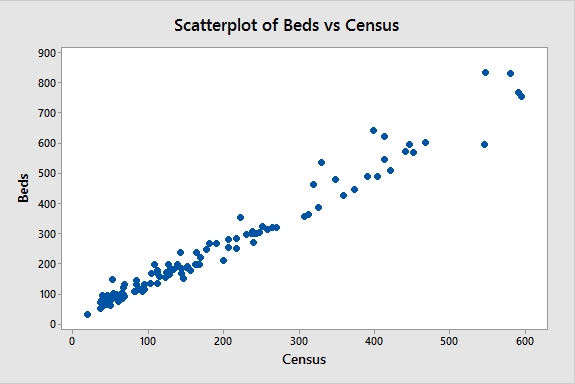
\includegraphics[scale=.5]{./images/scatterplot_beds-vs-census.png}
 % scatterplot_beds-vs-census.png: 575x384 pixel, 96dpi, 15.21x10.16 cm, bb=0 0 431 288
\end{figure}

\item
  \(InfctRsk = 3.716 + 0.002457 Beds\) \\ The \emph{p}-value of the
  regression is 0.000 which indicates a statistically significant linear
  relationship between the two variables.
\item
  \(InfctRsk = 3.697 + 0.003374 Census\) \\ The \emph{p}-value of the
  regression is 0.000 which indicates a statistically significant linear
  relationship between the two variables.
\item
  \(InfctRsk = -0.692 + 0.3157 Stay + 0.02050 Xray - 0.00019 Beds + 0.00216 Census\)

  \begin{enumerate}
  \def\labelenumii{\roman{enumii})}
  \tightlist
  \item
    The \emph{p}-value of the regression is 0.000, so we can conclude
    that there is a statistically significant relationship.
  \item
    The \emph{p}-value of beds is 0.950 so we can conclude that it is
    not statistically significant in this model.
  \item
    The \emph{p}-value of census is 0.587 so we can conclude that it too
    is not statistically significant in this model.
  \item
    The most likely reason that the significance results for beds and
    census changed from the simple model to the multiple model is that
    the other variables, xray and stay, were much better predictors of
    infection risk. Therefore, in the presence of these other
    predictors, beds and census did not have any significant effect on
    the residuals of the model.
  \end{enumerate}
\item
  \(InfctRsk = -0.701 + 0.3166 Stay + 0.02049 Xray + 0.001916 Census\)

  \begin{enumerate}
  \def\labelenumii{\roman{enumii})}
  \tightlist
  \item
    In this model, every predictor has a \emph{p}-value less than 0.05,
    so we can conclude that they are all statistically significant.
  \item
    The MSE for this model is 1.091. This is a bit lower than the MSE
    for the 4-variable model: 1.1017. This is evidence that the
    3-variable model is preferable, because it indicates less variation
    of the data points around the regression line.
  \end{enumerate}
\item
  The residual vs fit plot shows a random bounce of values around the
  residual = 0 line which indicates good linear fit and consistent
  variance of the error terms. The histogram shows a near normal
  distribution of the residuals which shows the error distribtion is
  close to normal.
  \begin{figure}[!h]
   \begin{floatrow}
    \ffigbox{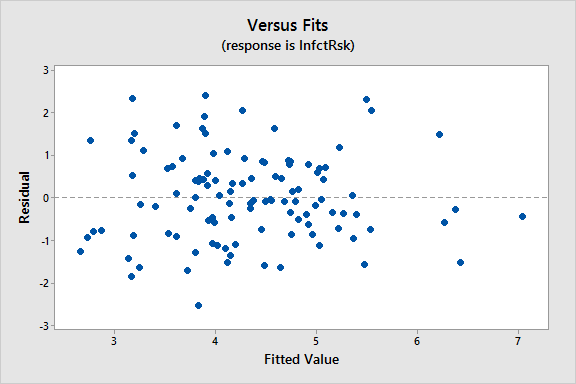
\includegraphics[scale=0.5]{./images/plot_3-variable-model_residual-vs-fitted.png}}{}
   \ffigbox{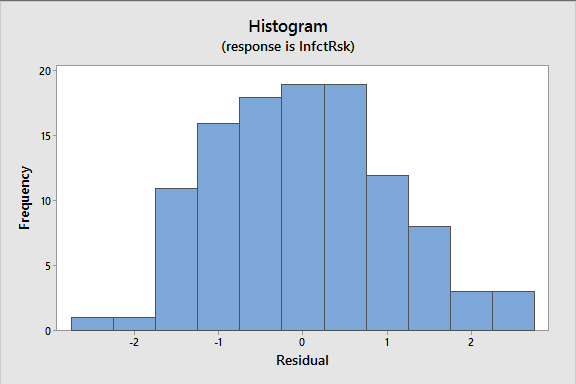
\includegraphics[scale=0.5]{./images/histogram_3-variable-model_residuals.png}}{}
  \end{floatrow}

  \end{figure}
  
\end{enumerate}

    \subsubsection{Question 3}\label{question-3}

\begin{enumerate}
\def\labelenumi{\alph{enumi})}
\tightlist
\item
  \(Y = 10.200 + 4.000 X\)
\end{enumerate}

    \begin{Verbatim}[commandchars=\\\{\}]
{\color{incolor}In [{\color{incolor}1}]:} \PY{c}{\PYZsh{} part (b)}
        \PY{k+kn}{import} \PY{n+nn}{numpy} \PY{k+kn}{as} \PY{n+nn}{np}
        \PY{k+kn}{from} \PY{n+nn}{numpy.linalg} \PY{k+kn}{import} \PY{n}{inv}
        
        \PY{n}{X} \PY{o}{=} \PY{n}{np}\PY{o}{.}\PY{n}{matrix}\PY{p}{(}\PY{p}{[}\PY{p}{[}\PY{l+m+mi}{1}\PY{p}{,}\PY{l+m+mi}{1}\PY{p}{]}\PY{p}{,} \PY{p}{[}\PY{l+m+mi}{1}\PY{p}{,}\PY{l+m+mi}{0}\PY{p}{]}\PY{p}{,} \PY{p}{[}\PY{l+m+mi}{1}\PY{p}{,}\PY{l+m+mi}{2}\PY{p}{]}\PY{p}{,} \PY{p}{[}\PY{l+m+mi}{1}\PY{p}{,}\PY{l+m+mi}{0}\PY{p}{]}\PY{p}{,} \PY{p}{[}\PY{l+m+mi}{1}\PY{p}{,}\PY{l+m+mi}{3}\PY{p}{]}\PY{p}{,} \PY{p}{[}\PY{l+m+mi}{1}\PY{p}{,}\PY{l+m+mi}{1}\PY{p}{]}\PY{p}{,} \PY{p}{[}\PY{l+m+mi}{1}\PY{p}{,}\PY{l+m+mi}{0}\PY{p}{]}\PY{p}{,} \PY{p}{[}\PY{l+m+mi}{1}\PY{p}{,}\PY{l+m+mi}{1}\PY{p}{]}\PY{p}{,} \PY{p}{[}\PY{l+m+mi}{1}\PY{p}{,}\PY{l+m+mi}{2}\PY{p}{]}\PY{p}{,} \PY{p}{[}\PY{l+m+mi}{1}\PY{p}{,}\PY{l+m+mi}{0}\PY{p}{]}\PY{p}{]}\PY{p}{)}
        \PY{n}{Y} \PY{o}{=} \PY{n}{np}\PY{o}{.}\PY{n}{matrix}\PY{p}{(}\PY{p}{[}\PY{p}{[}\PY{l+m+mi}{16}\PY{p}{]}\PY{p}{,} \PY{p}{[}\PY{l+m+mi}{9}\PY{p}{]}\PY{p}{,} \PY{p}{[}\PY{l+m+mi}{17}\PY{p}{]}\PY{p}{,} \PY{p}{[}\PY{l+m+mi}{12}\PY{p}{]}\PY{p}{,} \PY{p}{[}\PY{l+m+mi}{22}\PY{p}{]}\PY{p}{,} \PY{p}{[}\PY{l+m+mi}{13}\PY{p}{]}\PY{p}{,} \PY{p}{[}\PY{l+m+mi}{8}\PY{p}{]}\PY{p}{,} \PY{p}{[}\PY{l+m+mi}{15}\PY{p}{]}\PY{p}{,} \PY{p}{[}\PY{l+m+mi}{19}\PY{p}{]}\PY{p}{,} \PY{p}{[}\PY{l+m+mi}{11}\PY{p}{]}\PY{p}{]}\PY{p}{)}
\end{Verbatim}

    \begin{Verbatim}[commandchars=\\\{\}]
{\color{incolor}In [{\color{incolor}2}]:} \PY{c}{\PYZsh{} part b\PYZhy{}i)}
        \PY{n}{inv}\PY{p}{(}\PY{n}{X}\PY{o}{.}\PY{n}{transpose}\PY{p}{(}\PY{p}{)} \PY{o}{*} \PY{n}{X}\PY{p}{)}
\end{Verbatim}

            \begin{Verbatim}[commandchars=\\\{\}]
{\color{outcolor}Out[{\color{outcolor}2}]:} matrix([[ 0.2, -0.1],
                [-0.1,  0.1]])
\end{Verbatim}
        
    \begin{Verbatim}[commandchars=\\\{\}]
{\color{incolor}In [{\color{incolor}3}]:} \PY{c}{\PYZsh{} part b\PYZhy{}ii)}
        \PY{n}{b} \PY{o}{=} \PY{n}{inv}\PY{p}{(}\PY{n}{X}\PY{o}{.}\PY{n}{transpose}\PY{p}{(}\PY{p}{)} \PY{o}{*} \PY{n}{X}\PY{p}{)} \PY{o}{*} \PY{n}{X}\PY{o}{.}\PY{n}{transpose}\PY{p}{(}\PY{p}{)} \PY{o}{*} \PY{n}{Y}
        \PY{n}{b}
\end{Verbatim}

            \begin{Verbatim}[commandchars=\\\{\}]
{\color{outcolor}Out[{\color{outcolor}3}]:} matrix([[ 10.2],
                [  4. ]])
\end{Verbatim}
        
    \begin{Verbatim}[commandchars=\\\{\}]
{\color{incolor}In [{\color{incolor}4}]:} \PY{c}{\PYZsh{} part b\PYZhy{}iii)}
        \PY{n}{e} \PY{o}{=} \PY{n}{Y} \PY{o}{\PYZhy{}} \PY{n}{X} \PY{o}{*} \PY{n}{b}
        \PY{n}{e}
\end{Verbatim}

            \begin{Verbatim}[commandchars=\\\{\}]
{\color{outcolor}Out[{\color{outcolor}4}]:} matrix([[ 1.8],
                [-1.2],
                [-1.2],
                [ 1.8],
                [-0.2],
                [-1.2],
                [-2.2],
                [ 0.8],
                [ 0.8],
                [ 0.8]])
\end{Verbatim}
        
    \begin{Verbatim}[commandchars=\\\{\}]
{\color{incolor}In [{\color{incolor}5}]:} \PY{c}{\PYZsh{} part b\PYZhy{}iv)}
        \PY{n}{SSE} \PY{o}{=} \PY{n}{Y}\PY{o}{.}\PY{n}{transpose}\PY{p}{(}\PY{p}{)} \PY{o}{*} \PY{n}{Y} \PY{o}{\PYZhy{}} \PY{n}{b}\PY{o}{.}\PY{n}{transpose}\PY{p}{(}\PY{p}{)} \PY{o}{*} \PY{n}{X}\PY{o}{.}\PY{n}{transpose}\PY{p}{(}\PY{p}{)} \PY{o}{*} \PY{n}{Y}
        \PY{n}{SSE}
\end{Verbatim}

            \begin{Verbatim}[commandchars=\\\{\}]
{\color{outcolor}Out[{\color{outcolor}5}]:} matrix([[ 17.6]])
\end{Verbatim}
        
    \begin{Verbatim}[commandchars=\\\{\}]
{\color{incolor}In [{\color{incolor}6}]:} \PY{c}{\PYZsh{} part b\PYZhy{}v)}
        \PY{n}{MSE} \PY{o}{=} \PY{p}{(}\PY{n}{SSE} \PY{o}{/} \PY{p}{(}\PY{l+m+mi}{10} \PY{o}{\PYZhy{}} \PY{l+m+mi}{2}\PY{p}{)}\PY{p}{)}\PY{o}{.}\PY{n}{item}\PY{p}{(}\PY{l+m+mi}{0}\PY{p}{,}\PY{l+m+mi}{0}\PY{p}{)}
        \PY{n}{se\PYZus{}squared\PYZus{}b} \PY{o}{=} \PY{n}{MSE} \PY{o}{*} \PY{n}{inv}\PY{p}{(}\PY{n}{X}\PY{o}{.}\PY{n}{transpose}\PY{p}{(}\PY{p}{)} \PY{o}{*} \PY{n}{X}\PY{p}{)}
        \PY{n}{se\PYZus{}squared\PYZus{}b}
\end{Verbatim}

            \begin{Verbatim}[commandchars=\\\{\}]
{\color{outcolor}Out[{\color{outcolor}6}]:} matrix([[ 0.44, -0.22],
                [-0.22,  0.22]])
\end{Verbatim}
        
    \begin{Verbatim}[commandchars=\\\{\}]
{\color{incolor}In [{\color{incolor}7}]:} \PY{c}{\PYZsh{} part b\PYZhy{}vi)}
        \PY{n}{X\PYZus{}h} \PY{o}{=} \PY{n}{np}\PY{o}{.}\PY{n}{matrix}\PY{p}{(}\PY{p}{[}\PY{p}{[}\PY{l+m+mi}{1}\PY{p}{]}\PY{p}{,} \PY{p}{[}\PY{l+m+mi}{2}\PY{p}{]}\PY{p}{]}\PY{p}{)}
        \PY{n}{Y\PYZus{}hat} \PY{o}{=} \PY{n}{X\PYZus{}h}\PY{o}{.}\PY{n}{transpose}\PY{p}{(}\PY{p}{)} \PY{o}{*} \PY{n}{b}
        \PY{n}{Y\PYZus{}hat}
\end{Verbatim}

            \begin{Verbatim}[commandchars=\\\{\}]
{\color{outcolor}Out[{\color{outcolor}7}]:} matrix([[ 18.2]])
\end{Verbatim}
        
    \begin{Verbatim}[commandchars=\\\{\}]
{\color{incolor}In [{\color{incolor}8}]:} \PY{c}{\PYZsh{} part b\PYZhy{}vii)}
        \PY{n}{se\PYZus{}squared\PYZus{}Y\PYZus{}hat} \PY{o}{=} \PY{n}{X\PYZus{}h}\PY{o}{.}\PY{n}{transpose}\PY{p}{(}\PY{p}{)} \PY{o}{*} \PY{n}{se\PYZus{}squared\PYZus{}b} \PY{o}{*} \PY{n}{X\PYZus{}h}
        \PY{n}{se\PYZus{}squared\PYZus{}Y\PYZus{}hat}
\end{Verbatim}

            \begin{Verbatim}[commandchars=\\\{\}]
{\color{outcolor}Out[{\color{outcolor}8}]:} matrix([[ 0.44]])
\end{Verbatim}
        
    \begin{Verbatim}[commandchars=\\\{\}]
{\color{incolor}In [{\color{incolor}9}]:} \PY{c}{\PYZsh{} part (c)}
        \PY{n}{cov\PYZus{}b0\PYZus{}b1} \PY{o}{=} \PY{n}{se\PYZus{}squared\PYZus{}b}\PY{o}{.}\PY{n}{item}\PY{p}{(}\PY{l+m+mi}{0}\PY{p}{,}\PY{l+m+mi}{1}\PY{p}{)} \PY{c}{\PYZsh{} \PYZhy{}0.22}
        \PY{n}{s\PYZus{}b0} \PY{o}{=} \PY{n}{np}\PY{o}{.}\PY{n}{sqrt}\PY{p}{(}\PY{n}{se\PYZus{}squared\PYZus{}b}\PY{o}{.}\PY{n}{item}\PY{p}{(}\PY{l+m+mi}{0}\PY{p}{,}\PY{l+m+mi}{0}\PY{p}{)}\PY{p}{)}
        \PY{n}{s\PYZus{}b1} \PY{o}{=} \PY{n}{np}\PY{o}{.}\PY{n}{sqrt}\PY{p}{(}\PY{n}{se\PYZus{}squared\PYZus{}b}\PY{o}{.}\PY{n}{item}\PY{p}{(}\PY{l+m+mi}{1}\PY{p}{,}\PY{l+m+mi}{1}\PY{p}{)}\PY{p}{)}
        \PY{n}{corr\PYZus{}b0\PYZus{}b1} \PY{o}{=} \PY{n}{cov\PYZus{}b0\PYZus{}b1} \PY{o}{/} \PY{p}{(}\PY{n}{s\PYZus{}b0} \PY{o}{*} \PY{n}{s\PYZus{}b1}\PY{p}{)}
        \PY{n}{corr\PYZus{}b0\PYZus{}b1}
\end{Verbatim}

            \begin{Verbatim}[commandchars=\\\{\}]
{\color{outcolor}Out[{\color{outcolor}9}]:} -0.70710678118654746
\end{Verbatim}
        
    \subsubsection{Question 4}\label{question-4}

\begin{enumerate}
\def\labelenumi{\alph{enumi})}
\item
  \textbf{95.21\%} of the variation in degree liking (Y) is accounted
  for by moisture content (\(X_1\)) and sweetness (\(X_2\)).
\item
  The estimated standard deviation of the regression is
  \textbf{2.69330}.
\item
  The F-statistic of \textbf{129.08} with a p-value of \textbf{0.000}
  indicates that the model containing \(X_1\) and \(X_2\) is more useful
  in predicting Y than not taking into account the two predictors.
\item
  The t-statistic of \textbf{14.70} with a p-value of \textbf{0.000}
  indicates that the slope parameter for \(X_1\) is significantly
  different from 0 in this model.
\item
  The t-statistic of \textbf{6.50} with a p-value of \textbf{0.000}
  indicates that the slope parameter for \(X_2\) is significantly
  different from 0 in this model.
\item
  We estimate that E(Y) increases by \textbf{4.425} units when \(X_1\)
  increases by \textbf{1} unit and \(X_2\) is held constant.
\item
  We estimate that E(Y) increases by \textbf{4.375} units when \(X_2\)
  increases by \textbf{1} unit and \(X_1\) is held constant.
\item
  We predict that the degree of brand liking when moisture content is 7
  and sweetness is 3 is \textbf{81.75}.
\end{enumerate}


    % Add a bibliography block to the postdoc
    
    
    
    \end{document}
